\documentclass{uebblatt}

\begin{document}

\maketitle{1}{}
\marginpar{\vspace*{-1cm}\hspace*{-0.5cm}\href{http://poesophicalbits.blogspot.de/2013/05/lambda-calculus-and-category-theory-in.html}{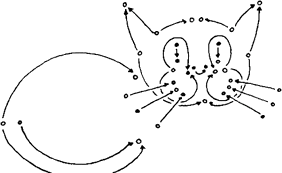
\includegraphics[angle=90,scale=0.5]{images/katzegorie}}}

\begin{aufgabe}{Beispiele für natürliche Transformationen}
Sei~$\Id_\Set : \Set \to \Set$ der Identitätsfunktor auf~$\Set$ und~$K : \Set
\to \Set$ der Funktor
\[ \begin{array}{@{}rrcl@{}}
  & X &\longmapsto& X \times X \\
  & f &\longmapsto& f \times f \defeq ((a,b) \mapsto (f(a),f(b))).
\end{array} \]
\begin{enumerate}
\item Zeige: Es gibt nur eine einzige natürliche Transformation $\eta : \Id_\Set
\to K$, nämlich die mit den Komponenten~$\eta_X : X \to X \times X,\ x \mapsto (x,x)$.

{\tiny
\emph{Tipp:} Betrachte zum Nachweis der Eindeutigkeit geeignete Abbildungen $1 \to X$, $\heartsuit
\mapsto x$. Dabei ist~$1 = \{\heartsuit\}$ eine einelementige Menge, das
\emph{einsame Herz}. \texttt{:-(}\par}
\item Wir nehmen an, dass wir für jede nichtleere Menge~$X$ ein bestimmtes
Element~$a_X \in X$ gegeben haben. Zeige:
Die Setzung
$\tau_X : X \to X,\ x \mapsto a_X$
definiert \emph{nicht} eine natürliche Transformation~$\Id_\C \to \Id_\C$,
wobei~$\C$ die Kategorie der nichtleeren Mengen und beliebigen Abbildungen
bezeichnet.
\item
Welche natürlichen Transformationen $\Id_\C \to \Id_\C$ gibt es,
wenn~$\C$ die Kategorie der reellen Vektorräume bezeichnet?
\item Seien~$\alpha, \beta : M \to N$ zwei Monoidhomomorphismen. Zeige, dass
die induzierten Funktoren zwischen den Kategorien~$BM$ und~$BN$ genau dann
isomorph sind, wenn es ein invertierbares Element~$u \in N$ gibt mit~$\beta(x) \circ u = u
\circ \alpha(x)$ für alle~$x \in M$.
\end{enumerate}
\end{aufgabe}

\begin{aufgabe}{Kanonizität der horizontalen Komposition}
Sei~$\eta : F \to G$ eine natürliche Transformation zwischen
Funktoren~$F,G : \C \to \D$ und~$\varepsilon : J \to K$ eine natürliche
Transformation zwischen Funktoren~$J,K : \D \to \E$. Zeige, dass die beiden
Möglichkeiten, die \emph{horizontale Komposition}~$\eta \star \varepsilon : J
\circ F \to K \circ G$ zu definieren, übereinstimmen:
\[ (\eta \star \varepsilon)_X \defeq K(\eta_X) \circ \varepsilon_{F(X)}
  \qquad
  (\eta \star \varepsilon)_X \defeq \varepsilon_{G(X)} \circ J(\eta_X)
\]
\end{aufgabe}
\vspace{-2em}

\begin{aufgabe}{Allgemeines zu Kategorienäquivalenzen}
\begin{enumerate}
\item Zeige mit allen Details: Ein Funktor~$F : \C \to \D$ definiert genau dann
eine Kategorien\-äquivalenz, wenn er volltreu und wesentlich surjektiv ist.
%d.\,h. wenn für alle Objekte~$X$ und~$Y$ von~$\C$ die Abbildungen~$\Hom_\C(X,Y)
%\to \Hom_\D(F(X),F(Y))$ bijektiv sind und wenn zu jedem Objekt~$Z$ von~$\D$ ein
%Objekt~$X$ von~$\C$ mit~$F(X) \cong Z$ existiert.
\item Zeige: Das Quasiinverse einer Kategorienäquivalenz ist eindeutig bis auf
eindeutige Isomorphie.
\end{enumerate}
\end{aufgabe}

\begin{aufgabe}{Die duale Kategorie der Kategorie der Mengen}
\begin{enumerate}
\item Zeige: In der Kategorie der Mengen ist jeder Morphismus ins initiale
Objekt ein Iso.
\item Zeige: In~$\Set^\op$ stimmt die Aussage aus~a) nicht.
\item Folgere: Die Kategorien~$\Set$ und~$\Set^\op$ sind nicht äquivalent.
\end{enumerate}
\begin{minipage}{0.87\textwidth}
\tiny Ein initiales Objekt in einer Kategorie ist ein Objekt~$X$, sodass es zu
jedem Objekt~$Y$ genau einen Morphismus $X \to Y$ gibt.
Wenn du noch Lust hast, dann zeige, dass der kontravariante
Potenzmengenfunktor eine Äquivalenz zwischen~$\Set^\op$ und der Kategorie der
vollständigen atomischen Heyting-Algebren definiert.\par
\end{minipage}
\end{aufgabe}

\marginpar{\vspace*{-2.3cm}\hspace*{-2cm}\href{https://staff.fnwi.uva.nl/s.sourabh/cats/}{
\includegraphics[scale=0.4]{images/doctor-cat}}}

\end{document}
